% Pen-and-paper worksheet for Module 1.
% Compile with: xelatex -interaction=nonstopmode exercise.tex   (run twice)
%
% Set in Charter 12pt rather than the 14pt hand face of the older sheets:
% Charter was drawn to stay legible small, and the sheet has to fit five parts
% without becoming a stack of paper. The hand face is kept for the title.
\documentclass[a4paper, 12pt]{extarticle}
\usepackage[top=0.8in, bottom=0.75in, left=0.85in, right=0.85in]{geometry}
\usepackage{amsmath}
\usepackage{amssymb}
\usepackage{array}
\usepackage{graphicx}
\usepackage{hyperref}
\usepackage{tcolorbox}
\usepackage{enumitem}
\usepackage{etoolbox}
\usepackage{tikz}
\usepackage{fontspec}
\usetikzlibrary{calc,positioning}
\definecolor{pltblue}{HTML}{1F77B4}

% Body: a readable, economical text face, guarded so the file still compiles
% on a machine that has none of them.
\IfFontExistsTF{Charter}{\setmainfont{Charter}}{
  \IfFontExistsTF{Iowan Old Style}{\setmainfont{Iowan Old Style}}{
    \IfFontExistsTF{Georgia}{\setmainfont{Georgia}}{}}}

% Title: the house hand face, if this machine has one.
\newcommand{\ppfont}{}
\IfFontExistsTF{Pretty Neat}{\renewcommand{\ppfont}{\fontspec{Pretty Neat}}}{
  \IfFontExistsTF{Humor Sans}{\renewcommand{\ppfont}{\fontspec{Humor Sans}}}{
    \IfFontExistsTF{Excalifont}{\renewcommand{\ppfont}{\fontspec{Excalifont}}}{}}}

\setlength{\parindent}{0pt}
\setlength{\parskip}{0.4em}
\raggedbottom

\newcommand{\ansline}{\underline{\hspace{0.98\textwidth}}}
\newcommand{\blank}[1][2cm]{\underline{\hspace{#1}}}

% The molab link printed on the hand-off page. Students type this by hand, so
% it has to stay short: change it here and nowhere else.
\newcommand{\molaburl}{\texttt{go.skojaku.com/m01lab}}

% A part heading.
\newcommand{\parthead}[2]{%
  \vspace{0.6em}
  {\large\bfseries Part #1 --- #2}\par
  \vspace{-0.4em}\rule{\textwidth}{0.8pt}\par
  \vspace{0.2em}}

% Centred fill-in cell.
\newcolumntype{C}[1]{>{\centering\arraybackslash}p{#1}}

% ---------------------------------------------------------------------------
% The map: seven Upstate New York highways over four cities. The cities sit
% where they really sit --- Ithaca west, Syracuse north, Binghamton south,
% Albany far east --- and every road on it is a road you can drive, so the
% figure reads as a road map rather than as an abstract graph. The degrees are
% Ithaca 3, Syracuse 4, Binghamton 4, Albany 3; US-11, added in 1(b), takes
% Syracuse and Binghamton to 5.
% ---------------------------------------------------------------------------
\tikzset{
  % Every road is drawn the same, so no line weight or colour suggests a
  % distinction that isn't there. Only the shields differ, as on a real map.
  road/.style     = {line width=3.6pt, black!62, line cap=round},
  ishield/.style  = {draw=pltblue!60!black, fill=pltblue, text=white,
                     font=\bfseries\scriptsize, rounded corners=1.6pt,
                     inner sep=2pt},
  nshield/.style  = {draw=black!65, fill=white, text=black,
                     font=\bfseries\scriptsize, rounded corners=1.6pt,
                     inner sep=2pt},
  city/.style     = {circle, fill=black, inner sep=0pt, minimum size=6.5pt},
  cityname/.style = {font=\bfseries, inner sep=3pt},
}
\newcommand{\nymap}{%
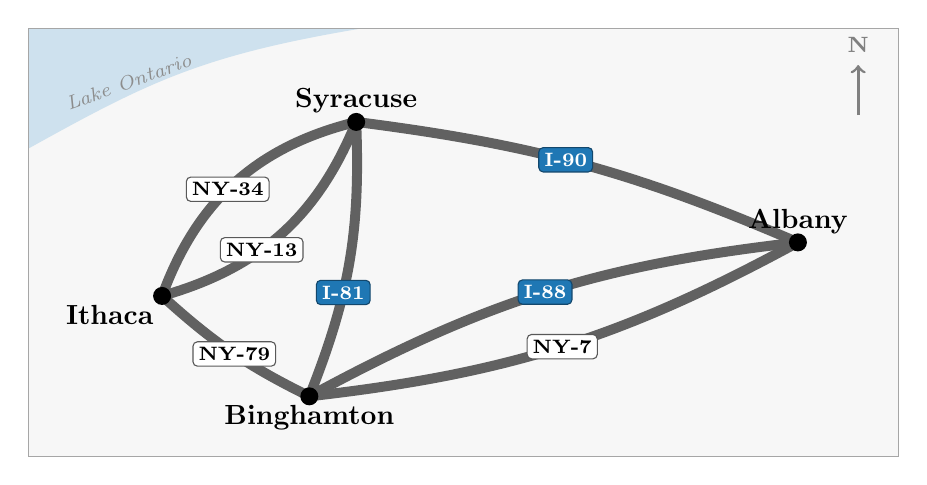
\begin{tikzpicture}[x=0.85cm, y=0.85cm]
    \begin{scope}
        \clip (0,0) rectangle (13,6.4);
        \fill[black!3] (0,0) rectangle (13,6.4);
        \fill[pltblue!22] (0,4.6) .. controls (1.8,5.6) and (2.6,6.0) ..
                          (5.0,6.4) -- (0,6.4) -- cycle;
    \end{scope}
    \node[font=\itshape\scriptsize, black!45, rotate=20] at (1.5,5.6)
        {Lake Ontario};

    \coordinate (I) at (2.0,2.4);
    \coordinate (S) at (4.9,5.0);
    \coordinate (B) at (4.2,0.9);
    \coordinate (A) at (11.5,3.2);

    \draw[road] (I) to[bend left=28]  (S);
    \draw[road] (I) to[bend right=26] (S);
    \draw[road] (I) to[bend right=8]  (B);
    \draw[road] (S) to[bend left=12]  (B);
    \draw[road] (S) to[bend left=8]   (A);
    \draw[road] (B) to[bend left=11]  (A);
    \draw[road] (B) to[bend right=11] (A);

    % Shields go on a second pass so no road is drawn across a number.
    \path (I) to[bend left=28]  node[nshield, pos=0.46] {NY-34} (S);
    \path (I) to[bend right=26] node[nshield, pos=0.40] {NY-13} (S);
    \path (I) to[bend right=8]  node[nshield, pos=0.52] {NY-79} (B);
    \path (S) to[bend left=12]  node[ishield, pos=0.62] {I-81}  (B);
    \path (S) to[bend left=8]   node[ishield, pos=0.46] {I-90}  (A);
    \path (B) to[bend left=11]  node[ishield, pos=0.50] {I-88}  (A);
    \path (B) to[bend right=11] node[nshield, pos=0.50] {NY-7}  (A);

    \node[city] at (I) {};  \node[cityname, below left] at (I) {Ithaca};
    \node[city] at (S) {};  \node[cityname, above] at (S) {Syracuse};
    \node[city] at (B) {};  \node[cityname, below] at (B) {Binghamton};
    \node[city] at (A) {};  \node[cityname, above] at (A) {Albany};

    \draw[->, black!50, line width=1pt] (12.4,5.1) -- (12.4,5.85);
    \node[font=\bfseries\footnotesize, black!50] at (12.4,6.15) {N};
    \draw[black!35] (0,0) rectangle (13,6.4);
\end{tikzpicture}}

% ---------------------------------------------------------------------------
% One city on its own, with #1 road-ends radiating out. #2 takes extra TikZ so
% the k=2 figure can ship with its pairing already drawn.
% ---------------------------------------------------------------------------
\newcommand{\landdeg}[2]{%
\begin{tikzpicture}[x=1cm, y=1cm]
    \path (-1.55,-1.55) rectangle (1.55,1.55);
    \foreach \i in {1,...,#1} {
        \pgfmathsetmacro\ang{90 - (\i-1)*360/#1}
        \draw[line width=2.6pt, black!72] (\ang:0.38) -- (\ang:1.18);
        \draw[thick, fill=white] (\ang:1.28) circle (0.1);
    }
    \draw[thick, fill=white] (0,0) circle (0.38);
    #2
\end{tikzpicture}}

\begin{document}

\begin{center}
{\ppfont\LARGE Drive Every Highway Once, Then Teach a Computer to Do It}
\end{center}

{\small Do this before the lecture, in pencil. Nothing here needs a word you
have not been given on the sheet.}

\parthead{1}{Seven highways}

Seven highways join four Upstate New York cities: \textbf{I}thaca,
\textbf{S}yracuse, \textbf{B}inghamton, \textbf{A}lbany. Drive every highway
exactly once.

\begin{center}
\nymap
\end{center}

{\bf Question 1(a)}: Find such a route. Start and finish anywhere. Cities may
repeat; highways may not. Write a city as its first letter and a highway as its
number. Two steps are done for you.

\vspace{0.4em}

I \; 13 \; S \; 34 \; I \; \blank[0.92cm] \; \blank[0.92cm] \; \blank[0.92cm]
\; \blank[0.92cm] \; \blank[0.92cm] \; \blank[0.92cm] \; \blank[0.92cm] \;
\blank[0.92cm] \; \blank[0.92cm] \; \blank[0.92cm]

\vspace{1.8cm}

{\bf Question 1(b)}: Draw an eighth highway on the map: \textbf{US-11},
Binghamton to Syracuse, alongside I-81. Try again. Which highway is left over?

\vspace{3.4cm}

\clearpage

{\bf Question 2}: One city, on its own. Arriving uses up one highway, leaving
uses up another --- so highways get used in \textbf{pairs}.

Join two road-ends with a curved line to mean ``in here, out there''. Pair up
as far as you can. The first is done.

\vspace{0.4em}

\begin{center}
{\setlength{\tabcolsep}{2pt}
\begin{tabular}{cccc}
\landdeg{2}{\draw[pltblue, dashed, line width=1.1pt] (90:1.28) to[out=0, in=0, looseness=2.6] (270:1.28);} &
\landdeg{3}{} &
\landdeg{4}{} &
\landdeg{5}{} \\
2 roads & 3 roads & 4 roads & 5 roads \\
\end{tabular}}
\end{center}

\vspace{0.3em}

\begin{center}
{\setlength{\tabcolsep}{9pt}
\begin{tabular}{|C{3.9cm}|C{1.9cm}|C{1.9cm}|C{1.9cm}|C{1.9cm}|}
\hline
 & \textbf{2 roads} & \textbf{3 roads} & \textbf{4 roads} &
\textbf{5 roads} \\
\hline
pairs you drew & 1 & & & \\[0.45cm] \hline
roads left over & 0 & & & \\[0.45cm] \hline
\end{tabular}}
\end{center}

\vspace{0.5em}

(a) Which ones can you drive straight \emph{through}? \blank[5cm]

(b) What do those numbers share? \blank[6cm]

(c) A left-over road has no partner, so this city must be the tour's
\blank[4.5cm]

\vspace{0.8em}

{\bf Question 3}: Count the highways at each city. Ithaca is done.

\begin{center}
{\setlength{\tabcolsep}{7pt}
\begin{tabular}{|C{3.4cm}|C{1.5cm}|C{1.5cm}|C{1.5cm}|C{1.5cm}|C{3.4cm}|}
\hline
 & \textbf{I} & \textbf{S} & \textbf{B} & \textbf{A} &
\textbf{how many have a left-over?} \\
\hline
seven roads & 3 & & & & \\[0.55cm] \hline
with US-11 too & & & & & \\[0.55cm] \hline
\end{tabular}}
\end{center}

\begin{minipage}{\textwidth}
One start, one finish. So at most \blank[1.2cm] cities may have a left-over
road.

\vspace{0.4em}

Seven roads: \blank[3.6cm] \hfill Eight roads: \blank[3.6cm] \hspace*{0.5cm}

\vspace{0.4em}

No route with eight because \underline{\hspace{8.5cm}}
\end{minipage}

\vspace{0.9em}

\begin{minipage}{0.53\textwidth}
{\bf Question 4}: The same puzzle, 1736. Königsberg: four pieces of land, seven
bridges. Two pairs join the same land; both of a pair must be crossed.

\vspace{0.6em}

Bridges: A \blank[0.9cm] B \blank[0.9cm] C \blank[0.9cm] D \blank[0.9cm]

\vspace{0.6em}

Is the walk possible? \blank[3.5cm]

\vspace{0.6em}

Destroying one bridge is enough. Which ones work? \blank[3cm]
\end{minipage}
\hfill
\begin{minipage}{0.42\textwidth}
\begin{center}
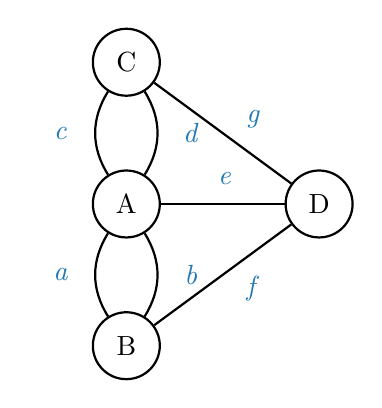
\begin{tikzpicture}[x=0.72cm, y=0.72cm, thick,
                    every node/.style={draw, circle, minimum size=0.85cm,
                                       inner sep=1pt, fill=white}]
    \node (C) at (0,2.5)   {C};
    \node (A) at (0,0)     {A};
    \node (B) at (0,-2.5)  {B};
    \node (D) at (3.4,0)   {D};
    \draw (A) to[bend left=32]  (B);
    \draw (A) to[bend right=32] (B);
    \draw (A) to[bend left=32]  (C);
    \draw (A) to[bend right=32] (C);
    \draw (A) -- (D);
    \draw (B) -- (D);
    \draw (C) -- (D);
    \node[draw=none, fill=none, pltblue] at (-1.15,-1.25) {\emph{a}};
    \node[draw=none, fill=none, pltblue] at ( 1.15,-1.25) {\emph{b}};
    \node[draw=none, fill=none, pltblue] at (-1.15, 1.25) {\emph{c}};
    \node[draw=none, fill=none, pltblue] at ( 1.15, 1.25) {\emph{d}};
    \node[draw=none, fill=none, pltblue] at ( 1.75, 0.45) {\emph{e}};
    \node[draw=none, fill=none, pltblue] at ( 2.25,-1.5)  {\emph{f}};
    \node[draw=none, fill=none, pltblue] at ( 2.25, 1.5)  {\emph{g}};
\end{tikzpicture}
\end{center}
\end{minipage}

\vspace{1em}

\parthead{2}{Three kinds of route}

A different network: five bus stops.

\begin{center}
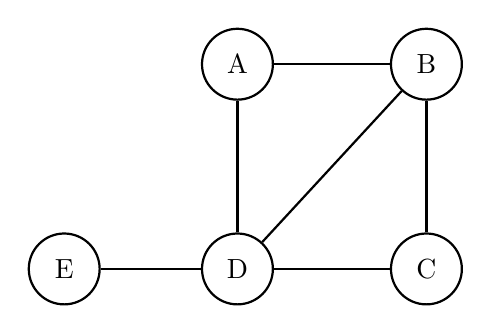
\begin{tikzpicture}[x=1cm, y=1cm, thick,
                    every node/.style={draw, circle, minimum size=0.9cm,
                                       inner sep=1pt, fill=white}]
    \node (A) at (0,1.6)   {A};
    \node (B) at (2.4,1.6) {B};
    \node (C) at (2.4,-1)  {C};
    \node (D) at (0,-1)    {D};
    \node (E) at (-2.2,-1) {E};
    \draw (A) -- (B);
    \draw (B) -- (C);
    \draw (C) -- (D);
    \draw (D) -- (A);
    \draw (B) -- (D);
    \draw (D) -- (E);
\end{tikzpicture}
\end{center}

{\bf Question 5(a)}: Fill in the table. First row done.

\begin{center}
{\setlength{\tabcolsep}{7pt}
\begin{tabular}{|C{3.4cm}|C{3.6cm}|C{3.4cm}|C{2.6cm}|}
\hline
\textbf{route} & \textbf{repeats a line?} & \textbf{repeats a stop?} &
\textbf{name} \\
\hline
A B D B C & yes (B--D twice) & yes (B) & \\[0.35cm] \hline
A B D C B & & & \\[0.5cm] \hline
A B C D E & & & \\[0.5cm] \hline
\end{tabular}}
\end{center}

{\bf Question 5(b)}: Write the right name in the last column.

\begin{tcolorbox}[colback=white, boxsep=1pt, top=3pt, bottom=3pt]
Repeats nothing: \textbf{path}. \quad Never repeats a line: \textbf{trail}.
\quad Repeats both: \textbf{walk}.
\end{tcolorbox}

{\bf Question 5(c)}: A route from A to E that repeats a stop but no line:

\vspace{0.3em}

A \blank[1.3cm] \blank[1.3cm] \blank[1.3cm] \blank[1.3cm] E

\vspace{0.9em}

{\bf Question 5(d)}: Your route in 1(a) is a \blank[3.5cm].

\vspace{0.6em}

{\bf Question 5(e)}: It cannot be a path: 7 lines need \blank[1.5cm] different
cities, and the map has \blank[1.5cm].

\vspace{0.9cm}

\parthead{3}{Predictions for the lab}

Fill this in on paper first, then check it in the lab. A new network:

\begin{center}
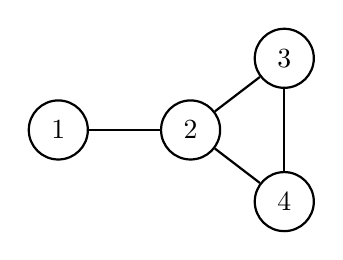
\begin{tikzpicture}[x=0.7cm, y=0.7cm, thick,
                    every node/.style={draw, circle, minimum size=0.75cm,
                                       inner sep=1pt, fill=white}]
    \node (1) at (-2.4,0)  {1};
    \node (2) at (0,0)     {2};
    \node (3) at (1.7,1.3) {3};
    \node (4) at (1.7,-1.3){4};
    \draw (1) -- (2);
    \draw (2) -- (3);
    \draw (2) -- (4);
    \draw (3) -- (4);
\end{tikzpicture}
\end{center}

\begin{minipage}[t]{0.46\textwidth}
{\bf Question 6(a)}: Write \textbf{1} in row $i$, column $j$ if a line joins
$i$ and $j$, else \textbf{0}. Row 1 done.

\vspace{0.4em}

\begin{center}
{\setlength{\tabcolsep}{4pt}
\begin{tabular}{r|C{0.85cm}|C{0.85cm}|C{0.85cm}|C{0.85cm}|}
\multicolumn{1}{c}{$A=$} & \multicolumn{1}{c}{1} & \multicolumn{1}{c}{2} &
\multicolumn{1}{c}{3} & \multicolumn{1}{c}{4} \\
\cline{2-5}
1 & 0 & 1 & 0 & 0 \\[0.1cm] \cline{2-5}
2 & & & & \\[0.28cm] \cline{2-5}
3 & & & & \\[0.28cm] \cline{2-5}
4 & & & & \\[0.28cm] \cline{2-5}
\end{tabular}}
\end{center}
\end{minipage}
\hfill
\begin{minipage}[t]{0.5\textwidth}
{\bf Question 6(b)}: Add up each row, then compare with the picture.

\vspace{0.5em}

row totals: \blank[1cm] \blank[1cm] \blank[1cm] \blank[1cm]

\vspace{0.6em}

Each row total is the \underline{\hspace{4.4cm}}

\vspace{0.9em}

of that node.
\end{minipage}

\vspace{1.2em}

{\bf Question 6(c)}: A \textbf{2-step route} is one line, then one more. Count
them on the picture.

\vspace{0.5em}

1 to 3: \; how many? \blank[1.2cm] \; list them: $1 \rightarrow$ \blank[1cm]
$\rightarrow 3$ \hspace*{2cm}

\vspace{1.1cm}

1 to 2: \; how many? \blank[1.2cm] \; why? \underline{\hspace{4.6cm}}

\vspace{1.1cm}

2 back to 2: \; how many? \blank[1.2cm]

\vspace{1.2cm}

{\bf Question 6(d)}: The lab will square your grid. What do you expect in
$A^2$?

\vspace{0.5em}

row 1, column 3: \blank[1.5cm] \qquad row 1, column 2: \blank[1.5cm]

\vspace{1.1cm}

the diagonal: \underline{\hspace{8cm}}

\vspace{1.3cm}

\begin{tcolorbox}[colback=white, boxsep=1pt, top=4pt, bottom=4pt]
\textbf{Now the lab, in pairs.} Bring this sheet. One laptop, two people: the
one not typing says the answer before the other one runs the cell.

\vspace{0.3em}

\begin{center}
\large \molaburl
\end{center}
\end{tcolorbox}

\end{document}
